\documentclass[a4paper]{article}

%% Language and font encodings
\usepackage[english]{babel}
\usepackage[utf8x]{inputenc}
\usepackage[T1]{fontenc}

\usepackage{listings}
\usepackage{graphicx}
\usepackage{rotating}
\usepackage{multirow}
\usepackage[toc,page]{appendix}
\usepackage{tikz}
\usetikzlibrary{arrows}
\usetikzlibrary{decorations.markings}
\usepackage{amsfonts,amstext,amsmath,amssymb}
\usepackage{flexisym}

\usepackage{array}
\usepackage{float}



\lstset{
    language=R,
    basicstyle=\footnotesize\ttfamily,
    keywordstyle=\color{blue},
    commentstyle=\ttfamily\color{dkgreen},
    backgroundcolor=\color{white},
    showspaces=false,
    showstringspaces=false,
    showtabs=false,
    tabsize=2,
    captionpos=b,
    breaklines=true,
    breakatwhitespace=false,
    title=\lstname,
    escapeinside={},
    keywordstyle={},
    morekeywords={}
    }

\DeclareMathOperator{\logis}{logis}
% Diverses commandes
\newcommand{\R}{\mathbb{R}}
\newcommand{\Rd}{\mathbb{R}^d}
\newcommand{\Rp}{\mathbb{R}^p}
\newcommand{\Xd}{\mathbb{X}^d}

% Diverses commandes
\newcommand{\calA}{{\cal A}}
\newcommand{\calB}{{\cal B}}
\newcommand{\calE}{{\cal E}}
\newcommand{\calF}{{\cal F}}
\newcommand{\calM}{{\cal M}}
\newcommand{\calN}{{\cal N}}
\newcommand{\calP}{{\cal P}}
\newcommand{\calT}{{\cal T}}
\newcommand{\calU}{{\cal U}}
\newcommand{\calW}{{\cal W}}
\newcommand{\calX}{{\cal X}}
\newcommand{\calZ}{{\cal Z}}


% Lettre ou chiffe en gras
\newcommand{\un}{\mathbf{1}}
\newcommand{\ba}{\mathbf{a}}
\newcommand{\bb}{\mathbf{b}}
\newcommand{\bc}{\mathbf{c}}
\newcommand{\bd}{\mathbf{d}}
\newcommand{\bg}{\mathbf{g}}
\newcommand{\bh}{\mathbf{h}}
\newcommand{\be}{\mathbf{e}}
\newcommand{\bL}{\mathbf{L}}
\newcommand{\bn}{\mathbf{n}}
\newcommand{\bp}{\mathbf{p}}
\newcommand{\bq}{\mathbf{q}}
\newcommand{\br}{\mathbf{r}}
\newcommand{\bs}{\mathbf{s}}
\newcommand{\bt}{\mathbf{t}}
\newcommand{\bu}{\mathbf{u}}
\newcommand{\bv}{\mathbf{v}}
\newcommand{\bW}{\mathbf{W}}
\newcommand{\bw}{\mathbf{w}}
\newcommand{\bx}{\mathbf{x}}
\newcommand{\bsx}{\boldsymbol{x}}
\newcommand{\bX}{\mathbf{X}}
\newcommand{\bsX}{\boldsymbol{X}}
\newcommand{\by}{\mathbf{y}}
\newcommand{\bsy}{\boldsymbol{y}}
\newcommand{\bY}{\mathbf{Y}}
\newcommand{\bsY}{\boldsymbol{Y}}
\newcommand{\bZ}{\mathbf{Z}}
\newcommand{\bz}{\mathbf{z}}
\newcommand{\bzero}{\mathbf{0}}

% Lettre grecque en gras % requiert \usepackage{amsbsy}
\newcommand{\balpha}{\boldsymbol{\alpha}}
\newcommand{\bbeta}{\boldsymbol{\beta}}
\newcommand{\bchi}{\boldsymbol{\chi}}
\newcommand{\bdelta}{\boldsymbol{\delta}}
\newcommand{\bDelta}{\boldsymbol{\Delta}}
\newcommand{\bepsilon}{\boldsymbol{\epsilon}}
\newcommand{\bGamma}{\boldsymbol{\Gamma}}
\newcommand{\bgamma}{\boldsymbol{\gamma}}
\newcommand{\blambda}{\boldsymbol{\lambda}}
\newcommand{\bkappa}{\boldsymbol{\kappa}}
\newcommand{\bmu}{\boldsymbol{\mu}}
\newcommand{\bnu}{\boldsymbol{\nu}}
\newcommand{\bpi}{\boldsymbol{\pi}}
\newcommand{\bphi}{\boldsymbol{\phi}}
\newcommand{\brho}{\boldsymbol{\rho}}
\newcommand{\bsigma}{\boldsymbol{\sigma}}
\newcommand{\bSigma}{\boldsymbol{\Sigma}}
\newcommand{\btheta}{\boldsymbol{\theta}}
\newcommand{\bTheta}{\boldsymbol{\Theta}}
\newcommand{\bvarepsilon}{\boldsymbol{\varepsilon}}
\newcommand{\bxi}{\boldsymbol{\xi}}


% Lettre verticale en gras  % requiert \usepackage{amsbsy}
\newcommand{\ve}[1]{{\boldsymbol{#1}}}
\newcommand{\x}{\boldsymbol{x}}
\newcommand{\X}{\boldsymbol{X}}
\newcommand{\z}{\boldsymbol{z}}
\newcommand{\Z}{\boldsymbol{Z}}


\newcommand{\argmin}{\mathop{\mathrm{argmin}}}
\newcommand{\argmax}{\mathop{\mathrm{argmax}}}
\newcommand{\trace}{\mathop{\mathrm{Tr}}}
\newcommand{\diag}{\mathop{\mathrm{diag}}}
\newcommand{\mix}{\textsc{mixmod}}
\newcommand{\II}{1 \! \! 1}
\newcommand{\IR}{\mathbb{R}}
\newcommand{\IZ}{\mathbb{Z}}
\newcommand{\IN}{\mathbb{N}}
\newcommand{\IE}{\mathbb{E}}
\newcommand{\mat}[4]{\begin{array}{cc}#1 & #2 \\#3 & #4 \end{array}}
\newcommand{\matb}[4]{\begin{array}{cc}{\bf #1} & {\bf #2} \\{\bf #3} & {\bf #4} \end{array}}
\newcommand{\med}{\mathrm{med}}
\newcommand{\tr}{\mbox{trace}}
\newcommand{\tra}[1]{\mbox{tr}{\bf #1}}
\newcommand{\var}{\mbox{var}}

\newcommand{\Esp}[1]{\mathbb{E}\left[#1\right]}
\newcommand{\Econd}[2]{\mathbb{E}\left[#1\left|#2\right.\right]}

\newcommand{\Prob}{\mathbb{P}}
\newcommand{\E}{\mathbb{E}}


\newtheorem{exmp}{Example}
\newtheorem{lemma}{Lemma}


%% Sets page size and margins
\usepackage[a4paper,top=3cm,bottom=2cm,left=3cm,right=3cm,marginparwidth=1.75cm]{geometry}

%% Useful packages
\usepackage{amsmath}
\usepackage{graphicx}
\usepackage[colorinlistoftodos]{todonotes}
\usepackage[colorlinks=true, allcolors=blue]{hyperref}

\title{Co-Clustering Binary Data Using Covariates}
\author{Serge Iovleff  \& Seydou Nourou Syllla \& Cheikh Loucoubar}

\begin{document}
\maketitle

\begin{abstract}
We present a novel co-clustering method using co-variates with application to genomic data.
\end{abstract}

\tableofcontents

\section{Introduction}

Classification is a method of data analysis that aims to group together a set of observations into homogeneous
classes. Its aim is the automatic resolution of problems by decision-making based on the observations induced to the
problems. Its main purpose is to define rules for classifying objects based on qualitative or quantitative variables
characterizing these objects. It plays an increasingly important role in many scientific and technical fields.
Clustering may be the most popular technique for data analysis in many disciplines.

Unlike classical clustering, which groups similar objects from a single collection of objects, coclustering or biclustering \cite{madeira2004biclustering} aims at simultaneously grouping objects from two disjoint sets, thus revealing interactions between elements of two sets. In recent years, co-clustering has been increasingly used
in many areas ranging from information retrieval, data mining, computer vision, biology, and so on.
It is most often used with bipartite spectral graphing partitioning methods in the field of \cite{Dhillon01}
extracting text data by simultaneously grouping documents and content (words) and analyzing huge corpora unlabeled
documents \cite{xu2010co} to simultaneously understand aggregates of subsets of web users(sessions) and information
from the page views.
Co-clustering algorithms have also been developed for computer vision applications.
it is used for grouping images by simultaneously grouping images with their low-level visual characteristics and for content-based image search \cite{guan2005spectral}\cite{rasiwasia2009holistic} \cite{ qiu2004image}.


% \begin{verbatim}[TODO]
% - Retrouver les SNP pertinents (analyse univariée ?) dans les blocs
% - Regarder les scores les plus élevés
% - Interpréter les blocs avec un coefficient \beta_1 très fort (en valeur absolue)
% - Tracer les bic pour 2 ou 3 groupes d'individus
% - Interpréter les blocs avec beaucoup de mutations
% \beta_0 + \beta_1 * Y_1 =i\log(\pi_i/(1-\pi_i))
% - Chercher des références sur l'interprétation de la régression logistique
% en médical (?)
% - tracer le temps d'execution
% - type="scores"
% \end{verbatim}
% \begin{verbatim}[]
% - Justifier le nombre de classes en lignes 
% - justifier le nombre de classes en colonnes
% - Choisir les classements les plus déterminants via le $\beta_1$ ou le OR
% - classer les Groupes de SNPs des plus déterminants aux moins déterminants
% ---- Trouver une méthode pour prédire Y en fonction des gènes de la meilleure classe
% ---- Faire de même pour les autres blocks de gènes
% ----- Faire un tableau résumé de ces resultats (Si on arrive a avoir que la meilleur classe de génes permet de mieux predire Y commparé aux autres classes on a gagné)

% \end{verbatim}

% The rest of the article is organized as follows. In Section~\ref{sec:BlockMixtureModels},
% we give the mathematical foundation (without going into detailed proofs) of latent block models
% for binary, contingency and continuous data-sets. In Section~\ref{sec:usingblockcluster},
% we elaborate various details of  blockcluster
% %\pkg{blockcluster} 
% package and illustrate its usage with the help of various examples.
% This part can also act as first-hand comprehensive tutorial for the audience who are interested in running the blockcluster
% % \pkg{blockcluster}
% package directly. Finally we illustrate our package on real data-sets in Section~\ref{sec:applications} and terminate with some concluding
% remarks in Section~\ref{sec:conclusion}.


\section{Block mixture models}
\label{sec:Block mixture models}
\subsection{Classical latent block model}
Let $\bx$ be a data set doubly indexed by a set $I$ with $n$ elements (individuals) and a set $J$ with $m$ elements (variables). We represent a
partition of $I$ into $g$ clusters by $\bz=(z_{11},\ldots,z_{ng})$ with
$z_{ik}=1$ if $i$ belongs to cluster $k$ and $z_{ik}=0$ otherwise, $z_i=k$
if $z_{ik}=1$ and we denote by $z_{.k}=\sum_i z_{ik}$ the cardinality of
row cluster $k$. Similarly, we represent a partition of $J$ into $d$ clusters
by $\bw=(w_{11},\ldots,w_{md})$ with $w_{j\ell}=1$ if $j$ belongs to cluster
$\ell$ and $w_{j\ell}=0$ otherwise, $w_j=\ell$ if $w_{j\ell}=1$ and we denote
$w_{.\ell}=\sum_j w_{j\ell}$ the cardinality of column cluster $\ell$.

The block mixture model formulation is  defined in \cite{Govaert2003} and
\cite{bhatia2014blockcluster} (among others) by the following probability
density function
$$f(\bx;\btheta)=\sum_{\bu \in \calU} p(\bu;\btheta) f(\bx|\bu;\btheta)$$
where $\calU$ denotes the set of all possible labellings of $I\times J$
and $\btheta$ contains all the unknown parameters of this model. By
restricting this model to a set of labellings of $I\times J$ defined by a
product of labellings of $I$ and $J$, and further assuming that the
labellings of $I$ and $J$ are independent of each other, one obtain the
decomposition
\begin{equation}
  \label{eq:latent_block_model}
  f(\bx;\btheta)=\sum_{(\bz,\bw) \in \cal{Z \times W}}
  p(\bz;\btheta) p(\bw;\btheta) f(\bx|\bz,\bw;\btheta)
\end{equation}
where $\calZ$ and $\calW$ denote the sets of all possible labellings $\bz$
of $I$ and $\bw$ of $J$. Equation (\ref{eq:latent_block_model}) define a \emph{Latent Block Model}.

\subsection{Latent block model for binary variables with co-variables: General formulation}
\label{sec:Latent Block model}
From now, we assume that $\bx$ is a binary data set. Let $\by$ represents a data-set (co-variables) of $\R^p$ indexed by $I$.
In order to take into account this set of co-variables the classical
block model formulation is extended to propose a block mixture model
defined by the following probability density function
\begin{equation}
\label{eq:co_latent_block_model}
 f(\bx,\by;\btheta)=\sum_{(\bz,\bw) \in \cal{Z \times W}}p(\bz;\btheta) p(\bw;\btheta)
  f(\bx| \by,\bz,\bw;\btheta)  f(\by| \bz;\btheta).
\end{equation}
By extending the latent class principle of local independence to our block model, each data pair $(x_{ij},\by_i )$ will be independent once $z_i$ and
$w_j$ are fixed. Hence we have
$$f(\bx,\by|\bz,\bw;\btheta)=\prod_{i,j} f(x_{ij}, \by_{i};\btheta).$$
We choose to model the dependency between $x_{ij}$ and $\by_i$ using the canonical link for binary response data
\begin{equation}\label{eq:link}
f(x_{ij}|\by_i,\bbeta_{z_iw_j})= \logis(\beta_{0,z_iw_j}+\bbeta_{z_iw_j}^T\by_i)^{x_{ij}} \, \left(1-\logis(\beta_{0,z_iw_j}+\bbeta_{z_iw_j}^T\by_i)\right)^{1-{x_{ij}}}
\end{equation}
with $(\beta_0,\bbeta_{k,l})\in\R^{p+1}$ and $\logis(x) = e^x/(1+e^x)$.
Each data point $\by_i$ will be independent once $z_i$ are fixed.
In the examples presented in section \ref{sec:Applications}, we choose 
$$
f(\by|\bz;\btheta )=  \prod_{i} \phi(\by_i;\bmu_{z_i},\bSigma_{z_{i}})
$$
with $\phi$ denoting the multivariate Gaussian density in $\Rp$.

In order to simplify the notation, we add a constant coordinate $1$ to vectors $\by_i$
and write $\bbeta_{k,l}$ in the later rather than $(\beta_{0,k,l},\bbeta_{k,l})$.

The parameters are thus $\btheta=(\bpi,\brho,\bbeta,\bmu,\bSigma)$, where
$\bpi=(\pi_1,\ldots,\pi_g)$, $\brho=(\rho_1,\ldots,\rho_d)$ are the vectors
of probabilities $\pi_k$ and $\rho_\ell$ that a row and a column belong to
the $k$th row component and to the $\ell$th column component respectively,
$\bbeta=(\bbeta_{kl})$ are the coefficients of the logistic function,
$\bmu$ and $\bSigma$ are the means and variances of the
Gaussian density. Summarizing, we obtain the latent block mixture model
with pdf
\begin{equation}
  \label{eq:latent_block_model_1}
  f(\bx,\by|\btheta)=\sum_{(\bz,\bw) \in \calZ \times \calW}
  \prod_{i,j} \pi_{z_i} \rho_{w_j} \logis(\by_i^T\bbeta_{z_i w_j})^{x_{ij}}
  \left(1-\logis(\by_i^T\bbeta_{z_i w_j})\right)^{1-x_{ij}}
  \phi(\by_i;\bmu_{z_{i}},\bSigma_{z_{i}}).
\end{equation}

Using above formulation, the randomized data generation process can be described by the four steps row labellings (R), column labellings (C), co-variable data generation (Y) and data generation (X) as follows:
\begin{enumerate}
\item[(R)] Generate the labellings $\bz=(z_1,\ldots,z_n)$ according to the
  distribution $\bpi=(\pi_1,\ldots,\pi_g)$.
\item[(C)] Generate the labellings $\bw=(w_1,\ldots,w_m)$ according to the
distribution $\brho=(\rho_1,\ldots,\rho_d)$.
\item[(Y)] Generate for $i=1,...,n$  vector $\by_{i}$ according to
the Gaussian distribution $\mathcal{N}_p(\bmu_{z_{i}},\bSigma_{z_{i}})$.
\item[(X)] Generate for $i=1,...,n$ and $j=1,...,m$ a value $x_{ij}$ according to the Bernoulli distribution $f(x_{ij}|\by_i;\bbeta_{z_i w_j})$
given in (\ref{eq:link}).
\end{enumerate}

\subsection{Model parameters estimation}
\label{sec:Model parameters estimation}
The complete data is represented as a vector $(\bx,\by,\bz,\bw)$
where unobservable vectors $\bz$ and $\bw$ are the labels. The log-likelihood to maximize is
\begin{equation}
  \label{eq:loglikelihood}
  l(\btheta)=\log f(\bx,\by;\btheta)
\end{equation}
and the double missing data structure, namely $\bz$ and $\bw$, makes statistical inference more difficult than usual. More precisely, if we try to use an EM algorithm as in standard mixture model \cite{Dempster} the complete data log-likelihood is find to be
\begin{equation}\label{eq:Lc_bloc_latent}
 L_C(\bz,\bw,\btheta)=\sum_k z_{.k} \log \pi_k + \sum_\ell w_{.\ell} \log \rho_\ell
  + \sum_{i,j,k,\ell} z_{ik}w_{j\ell}\log f(x_{ij},\by_i;\btheta_{k\ell}).
\end{equation}
The EM algorithm maximizes the log-likelihood $l(\btheta)$ iteratively by maximizing the conditional expectation $Q(\btheta,\btheta^{(c)})$ of the complete data log-likelihood given a previous current estimate
$\btheta^{(c)}$ and $(\bx,\by)$:
\begin{equation*}
  Q(\btheta,\btheta^{(c)})
  =\Econd{L_C(\bz,\bw,\theta)}{{\bx,\by,\btheta^{(c)}}}
  = \sum_{i,k}  t_{ik}^{(c)} \log \pi_k
  + \sum_{j,\ell} r_{j\ell}^{(c)} \log \rho_\ell
  + \sum_{i,j,k,\ell}  e_{ikj\ell}^{(c)} \log f(x_{ij},\by_i;\btheta_{k\ell})
\end{equation*}
where
\begin{equation*}
  t_{ik}^{(c)}=P(z_{ik}=1|\bx,\by,\btheta^{(c)}), \qquad
  r_{jl}^{(c)}=P(w_{j\ell}=1|\bx,\by,\btheta^{(c)}), \qquad
  e_{ikj\ell}^{(c)} = P(z_{ik}w_{j\ell}=1|\bx,\by, \btheta^{(c)})
\end{equation*}
Unfortunately, difficulties arise owing to the dependence structure in the model, in particular to determinate $e_{ikj\ell}^{(c)}$. The assumed independence of $\bz$ and $\bw$ in (\ref{eq:latent_block_model}) is not preserved by the posterior probability.

To solve this problem an approximate solution is proposed in \cite{Govaert2003} using the \cite{hathaway_86b} and \cite{neal_98} interpretation of the VEM algorithm. Consider a family of probability distribution $q(z_{ik},w_{j\ell})$ verifying $q(z_{ik},w_{j\ell})>0$ and the relation $q(z_{ik},w_{j\ell}) =q(z_{ik}) q(w_{j\ell})$, for all $i,j,k,l$. Set $t_{ik} =q(z_{ik})$
and $r_{jl} = q(w_{j\ell})$, $\bt=(t_{ik})_{ik}$ for $i=1,\ldots,n$, $k=1,\ldots,g$ and
$\br=(r_{jl})_{jl}$ for $j=1,\ldots,m$ and $l=1,\ldots,d$. Using the concavity of the $\log$ function, one shows easily that
\begin{equation}
 l(\btheta) \geq \tilde{F}_C(\bt,\br;\btheta) +
 KL(q(\bz,\bw)\parallel p(\bz,\bw|\bx,\by, \btheta))
\end{equation}
with $KL(q\parallel p)$ denoting the Kullback-Liebler divergence of distribution $p$ and $q$,
\begin{equation} \label{eq:fuzzycriterion}
\tilde{F}_C(\bt,\br;\btheta)=\sum_k t_{.k}\log \pi_k + \sum_{\ell} r_{.\ell} \log\rho_l +\sum_{i,j,k,\ell} t_{ik}r_{j\ell}\log f(x_{ij},\by_i;\btheta_{k\ell})  + H(\bt) + H(\br)
\end{equation}
and $H(\bt)$, $H(\br)$ denoting the entropy of $\bt$ and $\br$, i.e.
\begin{equation*}
H(\bt) = \sum_{ik} t_{ik}\log t_{ik},\qquad H(\br) = \sum_{jl} r_{jl}\log r_{jl}  .
\end{equation*}
$ \tilde{F}_C$ is called the free energy or the fuzzy criterion. As the Kullback-Liebler divergence is always positive, the fuzzy criterion is a lower bound of the log-likelihood and is use in replacement of it. Doing that, the maximization of the likelihood  $l(\btheta)$ is
replaced by the following problem
$$
\argmax_{\bt,\br,\btheta} \tilde{F}_C(\bt,\br,\btheta).
$$
This maximization can be achieved using the BEM algorithm detailed in next section.

\subsection{Block expectation maximization (BEM) Algorithm}

%Here we give brief outline of two algorithms used in our package. 
%
%\subsubsection{Block expectation maximization (BEM) algorithm}

The fuzzy clustering criterion given in (\ref{eq:fuzzycriterion})
can be maximized using a variational EM algorithm (VEM).
We here outline the various expressions evaluated during E and M steps.
\paragraph{E-Step:} we compute either the values of $\bt$ (respectively $\br$)
with $\br$ (respectively $\bt$) and $\btheta$ fixed. Details are given in
appendix \ref{app:EStep}.
\paragraph{M-Step:} we calculate row proportions $\bpi$ and column proportions $\brho$.
The maximization of $\tilde{F}_C$ w.r.t. $\bpi$, and w.r.t $\brho$, is obtained by maximizing
$\sum_k t_{.k}\log \pi_k $, and $\sum_\ell r_{.\ell}\log \rho_\ell$ respectively, which leads to
\begin{equation}\label{eq:prop-estimate}
\pi_k=\frac{t_{.k}}{n} \quad \textrm{ and } \quad \rho_\ell=\frac{r_{.\ell}}{m}.
\end{equation}
Also the estimate of model parameters $\bbeta$ will be obtained by maximizing
\begin{equation}\label{eq:betakl-estimate}
\bbeta_{kl}= \argmax_{\bbeta}\sum_{ij}t_{ik}r_{jl}\log f(x_{ij}|\by_i;\bbeta),\quad k=1,\ldots,g,\quad l=1,\ldots,d.
\end{equation}
(see appendix \ref{app:MStep} for details) and the parameters of the Gaussian
density by the usual formulas
\begin{equation}\label{eq:gauss-estimate}
\bmu_k = \frac{1}{t_{.k}} \sum_{i} t_{ik} \by_i
\qquad \mbox{ and } \qquad
\bSigma_k = \frac{1}{t_{.k}} \sum_{i} t_{ik} (\by_i -\bmu_{k})(\by_i - \bmu_{k})^T.
\end{equation}
\paragraph{BEM algorithm:} Using the {\bf E} and {\bf M} steps defined above, {\bf BEM} algorithm can be enumerated as follows:
\begin{description}
\item[Initialization] Set $\bt^{(0)},\br^{(0)}$ and $\btheta^{(0)}=(\bpi^{(0)},\brho^{(0)},\bbeta^{(0)},\bmu^{(0)}$, $\bSigma^{(0)}).$
\item[(a) Row-EStep] Compute $\bt^{(c+1)}$ using formula
\begin{equation}\label{eq:RowEStep}
t_{ik}^{(c+1)} = \displaystyle\frac{\pi_k^{(c)} \displaystyle\prod_{jl} \left(f(x_{ij}|\by_i;\bbeta_{kl}^{(c)})\phi(\by_i;\bmu_{k}^{(c)},\bSigma_{k}^{(c)})\right)^{r_{jl}^{(c)}} }
              {\sum_k \pi_k^{(c)} \displaystyle\prod_{jl}\left(f(x_{ij}|\by_i;\bbeta_{kl}^{(c)})\phi(\by_i;\bmu_{k}^{(c)},\bSigma_{k}^{(c)})\right)^{r_{jl}^{(c)}}}.
\end{equation}
\item[(b) Row-MStep] Compute $\bpi^{(c+1)}$, $\bmu^{(c+1)}$,  $\bSigma^{(c+1)}$ using equations (\ref{eq:prop-estimate}) and (\ref{eq:gauss-estimate}) and estimate
$\bbeta^{(c+1/2)}$ by solving maximization problem (\ref{eq:betakl-estimate}).
\item[(c) Col-EStep] Compute $\br^{(c+1)}$ using formula
\begin{equation}\label{eq:ColEStep}
r_{jl}^{(c+1)} = \frac{\rho_l^{(c)} \displaystyle\prod_{ik} f(x_{ij}|\by_i;\bbeta_{kl}^{(c+1/2)} )^{t_{ik}^{(c+1)}} }
              {\sum_l \rho_l^{(c)} \displaystyle\prod_{ik} f(x_{ij}|\by_i;\bbeta_{kl}^{(c+1/2)})^{t_{ik}^{(c+1)}}}.
\end{equation}
Observe that $r_{jl}$ does not depend of the density of $\by$.
\item[(d) Col-MStep] Compute $\brho^{(c+1)}$ using equations (\ref{eq:prop-estimate}) and estimate $\bbeta^{(c+1)}$ by solving maximization problem (\ref{eq:betakl-estimate}). 
\item[Iterate] Iterate {\bf (a)-(b)-(c)-(d)} until convergence.
\end{description}

\subsection{Selecting the number of blocks}

BIC is an information criterion defined as an asymptotic approximation of the logarithm of the integrated likelihood
(\cite{schwarz1978estimating}). The standard case leads to
write BIC as a penalised maximum likelihood:
$$
\mathrm{BIC} = -2\max_{\btheta} l(\btheta) + D \log(n)
$$
where $n$ is the number of statistical units and $D$ the number
of free parameters and $l(\btheta)$ defined in (\ref{eq:loglikelihood}).
Unfortunately, this approximation cannot be
used for LBM, due to the dependency structure of the observations
$(\bx,\by)$. However, a heuristic have been stated to define BIC
in \cite{keribin2012model} and \cite{keribin2015estimation}.
BIC-like approximations ICL lead to the following approximation
as $n$ and $m$ tend to infinity
\begin{equation}
\mathrm{BIC}(g,d) = -2\max_{\btheta}\log f(\bx, \by;\btheta) + (g-1)\log n  + \lambda\log n
+ (d-1)\log m + gd(p+1) \log(mn)
\end{equation}
with $\lambda$ the number of parameters of the $\by$ distribution.
For LBM, the intractable likelihood $f(\bx, \by;\btheta)$ is replaced by the maximized
free energy $\tilde{F}_C$ in (\ref{eq:fuzzycriterion}) obtained by the BEM algorithm.

\subsection{Measuring Influence of a Variable}

Let $j$ be fixed (a column of the matrix $\bx$). We would like to 
measure the effect of the variable
$\bx^j=(x_{ij})_{i=1}^n$ on $\by$. It is possible to obtain a measure
of this efffect by looking to the
posterior probability of $\by$.
\begin{lemma}
Let $(\bx,\bz,\bw)$ fixed. For $l=1,\ldots,d$ let $m_{l}$ denotes the number of columns with label $l$,
i.e $m_l = \#\{w_{jl} = 1,\; j=1,\ldots m\}$ and for a row $i$ fixed let $m_{il}$ denotes the number of
elements such that ${w_{jl} = 1}$ and $x_{ij} =1$, i.e. $m_{il}=\#\{w_{jl}x_{ij} = 1,\; j=1,\ldots m\}$.
The posterior probability of the co-variable $\by$ is
\begin{align}\label{eq:co-posterior-row}
f(\by|\bx,\bz,\bw,\btheta) & \propto \prod_{i=1}^n \prod_{l=1}^{d} \pi_{z_i} \rho_{l}^{m_l}
  \logis(\by_i^T\bbeta_{z_i l})^{m_{il}}
  \left(1-\logis(\by_i^T\bbeta_{z_i l})\right)^{m_l-m_{il}}
  \phi(\by_i;\bmu_{z_{i}},\bSigma_{z_{i}}) \nonumber \\
  & \propto \prod_{i=1}^n  \pi_{z_i} \phi(\by_i;\bmu_{z_{i}},\bSigma_{z_{i}})
           \prod_{l=1}^{d} \rho_{l}^{m_l}   
  \frac{e^{m_{il}\by_i^T\bbeta_{z_i l}}}{\left(1+e^{\by_i^T\bbeta_{z_i l}} \right)^{m_l}}
\end{align}
Alternatively, for $k=1,\ldots,g$, let $n_k$ denotes the number of rows with label $k$,
i.e. $n_k = \#\{z_{ik}=1, i=1,\ldots,n\}$. The posterior probability of the co-variable $\by$
is
\begin{equation}\label{eq:co-posterior-col}
f(\by|\bx,\bz,\bw,\btheta)  \propto \prod_{j=1}^m \rho_{w_{j}}
\prod_{k=1}^{g} \pi_{k}^{n_j} \prod_{i:z_i=k} \logis(\by_i^T\bbeta_{k w_j})^{x_{ij}}
  \left(1-\logis(\by_i^T\bbeta_{k w_j})\right)^{1-x_{ij}}
  \phi(\by_i;\bmu_{k},\bSigma_{k}).
\end{equation}
\end{lemma}
The proof of this lemma is straightforward and therefore omitted.

Assuming $\bz$ and $\bw$ known, we measure the influence of variable 
using its contribution to the posterior probability. Fixing $j$,
taking the logarithm and eliminating terms independant of
$\bx^j$, we obtain the \textit{influence measure criteria}
\begin{align}
I(j)& = \log\rho_{w_{j}} +\sum_{i=1}^n {x_{ij}}\log\logis(\by_i^T\bbeta_{z_i  w_j})
 +\sum_{i=1}^n {(1-x_{ij})}\log\left(1-\logis(\by_i^T\bbeta_{z_i w_j})\right) \nonumber \\
 &  = \log\rho_{w_{j}} + \sum_{i=1}^n \left( x_{ij} \by_{i}^{T}\bbeta_{z_i w_j} - \log({1+\exp(\by_{i}^{T}.\bbeta_{z_i w_j})}) \right).
\end{align}
Replacing the unknown labels $w_j$ and $z_i$ by there MAP estiamtors  $\hat{w}_j$ and $\hat{z}_i$, we
can sort the variables from the most to the less influential.

\section{Examples}\label{sec:Applications}
  \subsection{Simulated data}\label{subsec:SimulatedData}
%\textbf{Date de génération:}
We compute 80 times the accuracy and the elapsed time of the model for various configurations of the parameter
on a HP Zbook G3. The (averaged) computing time for different values of $n$ is given in the figure below
\begin{figure}[H]%[!htb]
\begin{center}
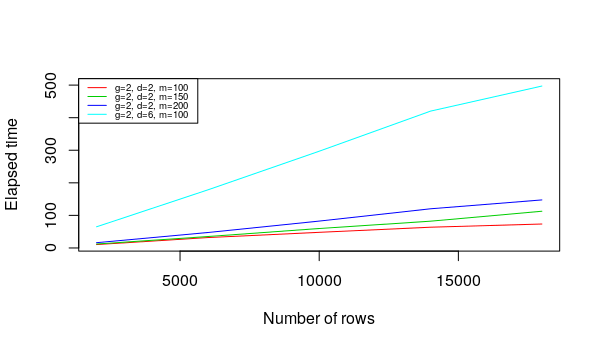
\includegraphics[width=12cm]{image_plots/times}
\end{center}
\caption{computational elapsed time for $n=$ 2000, 6000, 10000, 14000 and 18000 (in minutes)}
\label{fig:time}
\end{figure}
We can observe that as $n$ grow the elapsed time grow linearly, but that the slope increases as $d$ (the number
of class in columns) is increased.
The averaged well classified rate for these data is given in the table below with the standard deviation

\begin{table}[!htb]
    \centering
\begin{tabular}{|r|r|r|c|c|}
\hline
$d$ & $m$ & $n$  & Well classified rows & Well classified Columns \\
\hline
 2 &100 & 2000 & 0.9091250 & 0.9626562\\
 2 &100 & 6000 & 0.9027500 & 0.9444604\\
 2 &100 &10000 & 0.9207500  & 0.9618788\\
 2 &100 &14000 & 0.8928750 & 0.9451339\\
 2 &100 &18000 & 0.8875000 & 0.9498715\\
\hline
 2 &150 & 2000 & 0.9030833 &  0.9773625 \\
 2 &150 & 6000 & 0.9165000 &  0.9542896\\
 2 &150 &10000 & 0.9358333 & 0.9732000\\
 2 &150 &14000 & 0.9035833 & 0.9731152\\
 2 &150 &18000 & 0.9408333 &  0.9771382\\
\hline
 2 &200 & 2000 & 0.9345000 & 0.9770188\\
 2 &200 & 6000 & 0.8940000 & 0.9568625\\
 2 &200 &10000 & 0.9011875 & 0.9722437\\
 2 &200 &14000 & 0.9170000 & 0.9663027\\
 2 &200 &18000 & 0.9058125 & 0.9755889\\
\hline
 6 &100 & 2000 & 0.8535000 & 0.7367750\\
 6 &100 & 6000 & 0.8836250 &  0.7706229\\
 6 &100 &10000 & 0.8920000 & 0.8069587 \\
 6 &100 &14000 & 0.8982500 & 0.7922634\\
 6 &100 &18000 & 0.8565000         & 0.7899250\\
\hline
    \end{tabular}
    \caption{Estimated Proportions of Well-Classified rows and columns for $g=2$ and various configurations of $d,m,n$. Estimations
    were replicated 80 times.}
    \label{tab:classif}
\end{table}
  

% we simulated a matrix of 500 rows and 3000 columns and a co-variable vector of 500 lines following the normal law of parameters (sigma, variance).
% On this matrix, we simulated for 2 clusters in rows and 10 clusters in columns.
% To evaluate the parameters, we took a number of iterations equal to 10 and a 20 the number of convergence iterations of the algorithm.

% This simulation shows that the more we increase the number of columns, the longer the calculation time becomes (cf figure \ref{Runtime_evolution}). 

% \begin{figure}[!ht]
% \begin{center}
% 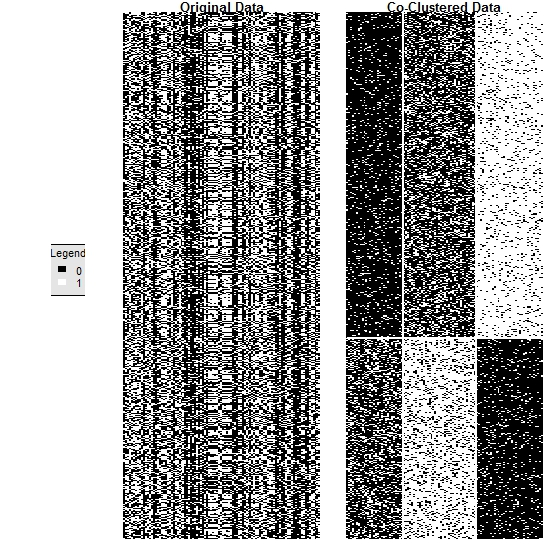
\includegraphics[width=4cm]{image_plots/coclusterbinary}
% \end{center}
% \caption{clustering picture }
% \end{figure}

 \subsection{Real Data Analysis}\label{subsec:RealData}
 % Cette partie sera fait par Cheikh Loucoubar

We consider the genetic data used by (\cite{loucoubar2016detecting}) and use this to compare the co-clustering with co-variable
and the co-clustering without co-variable. 
The genetic data gave a $515721$ SNPs and $455$ individulas. The quantitative phenotype represents
an individual falciparum attack(ipfa) for each individu({ \cite{loucoubar2016detecting}). The SNPs are coded in dominante. 

The groups on the lines are divided in two parts:  the susceptibility composed of a group of individuals with a positive IPFA and the  resistant ones composed of a group of individuals with a negative IPFA value.
We can take into account or not the mixture on the target variable in the proposed model. 

% \subsubsection{BIC Selection Criterion}\label{subsec:RealDataBIc}
 In this part we are interested in the performance of the selection criterion BIC for choosing the number of partitions in columns. We have 515721 variables, we have evaluated from 2  to 30 partitions and the penalized BIC suggests 14 partitions in columns
 (cf figure \ref{BIC}). 
 
 
 
\begin{figure}[!ht]
\begin{center}
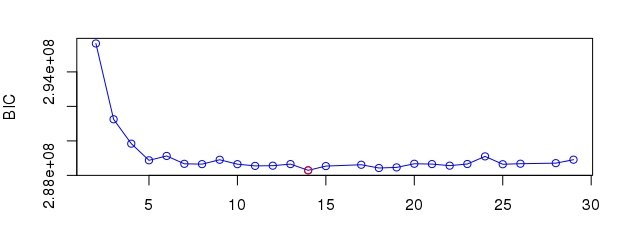
\includegraphics[width=10cm, scale=2.0]{image_plots/BIC_article.jpeg}
\end{center}
\caption{BIC Results}
\label{BIC}
\end{figure}

%\subsubsection{BIC Selection Criterion}\label{subsec:RealDataBIc}
The proportion of mutations in each block are given below
\begin{figure}[!ht]
\begin{center}
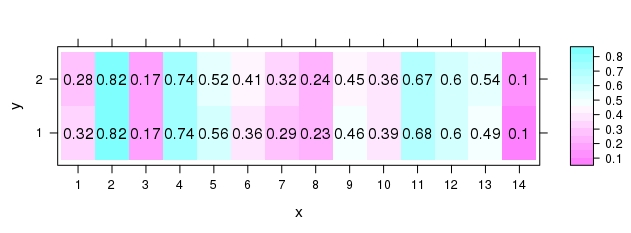
\includegraphics[width=10cm, scale=1.0]{image_plots/levelplot_co_clust.jpeg}
\end{center}
\caption{Percent of ones in each blocks}
\label{precent_ones}
\end{figure}




 
 
 
 
 
 
 
 
 
 
 















  
  
\section{Conclusion}\label{sec:conclusion}
\bibliographystyle{alpha}
\bibliography{sample}


\appendix
\section{Computing the (rows and columns) E-Step}
\label{app:EStep}
For the E-Step $t_{ik}$ value maximize the fuzzy criterion
given in equation (\ref{eq:fuzzycriterion}). Derivative with
respect to $t_{ik}$ gives
$$
\frac{\partial\tilde{F}_C(\bt,\br;\btheta)}{\partial t_{ik}} = \log\pi_k + \sum_{j,\ell} r_{j\ell} \log f_{k\ell}(x_{ij},\by_i;\btheta) - \log t_{ik} - 1.
$$
Equating this equation to zero, taking exponential and recalling that
$\sum_k t_{ik} = 1$, we obtain that $t_{ik}$ is updated as  
$$t_{ik}^{(c+1)}=\frac{\pi_{k}^{(c)}  \prod_{j,l}  \left[  f(x_{ij},\by_i;\btheta^{(c)})\right]^{r_{jl}^{(c)}}  }{ \sum_{k}\prod_{j,l}  \left[  f(x_{ij},\by_i;\btheta^{(c)})\right]^{r_{jl}^{(c)}}}.
$$
For numerical reason, we prefer to compute the logarithm of this expression which is
$$\log(t_{ik}^{(c+1)}) \propto \log(\pi_{k}^{(c)}) + \sum_{j,l} r_{jl}^{(c)} \log f(x_{ij},\by_i;\btheta^{(c)} ). $$
Recall that (see equation \ref{eq:link})
\begin{eqnarray*}
   \log f(x_{ij}|\by_i;\bbeta_{kl}^{(c)}) & = & x_{ij}\log(\logis(\by_{i}^{T}\bbeta_{kl}^{(c)}))
+ 
(1-x_{ij})\log(1-\logis(\by_{i}^{T}\bbeta_{kl}^{(c)})) \\
   & = & \log(1-\logis(\by_{i}^{T}\bbeta_{kl}^{(c)})) + x_{ij}\log\left(\frac{\logis(\by_{i}^{T}\bbeta_{kl}^{(c)})}{1-\logis(\by_{i}^{T}.\bbeta_{kl})}\right) \\
   & = & \log(1+\exp(\by_{i}^{T}\bbeta_{kl}^{(c)})) + x_{ij} \by_i^T\bbeta_{kl}^{(c)}
\end{eqnarray*}
giving
$$
\log t_{ik}^{(c+1)} \propto \log \pi_{k}^{(c)} + \sum_{j,l} r_{jl}^{(c)} x_{ij} \by_i^T.\bbeta_{kl}^{(c)}
- \sum_{l} r_{.l}^{(c)} \log(1+e^{\by_i^T.\bbeta_{kl}^{(c)}}) + m\;\log\phi(\by_i;\bmu_k^{(c)},\bSigma_k^{(c)}).
$$
Similar computation gives for $r_{jl}$
$$
\log(r_{jl}^{(c+1)}) \propto \log\left(\rho_{l}^{(c)}\right)
+ \sum_{i,k} t_{ik}^{(c+1)} \left( x_{ij} \by_i^T\bbeta_{kl}^{(c+1/2)} - 
\log\left(1+e^{\by_i^T.\bbeta_{kl}^{(c+1/2)}}\right) \right).
$$
Observe that the Gaussian distribution does not depend of $j$ nor $l$.
This term become constant when summing over $i$ and $k$ and disappears
when $r_{jl}$ values are normalized.

\section{Computing the M-Step}
\label{app:MStep}
For the M-Step, we use a Newton-Raphson algorithm in order to solve the equation (\ref{eq:betakl-estimate}). For each pair $(k,l)$ the function to maximize 
can be written
$$
\ell_{k,l}(\bbeta)=\sum_{i,j}\left( r_{jl}t_{ik}x_{ij} \by_{i}^{T}\bbeta- r_{jl}t_{ik}\log({1+\exp(\by_{i}^{T}.\bbeta)})\right) 
$$
The first derivative with respect to the d-th coordinate $\beta_d$ is
$$
\frac{\partial \ell_{k,l}(\beta)}{\partial \beta_{d}}= 
\sum_{i,j}\left( r_{jl}t_{ik}x_{ij}y_{i,d}- r_{jl}t_{ik} y_{i,d} \frac{\exp(\by_{i}^{T}\bbeta)}{1+\exp(\by_{i}^{T}\bbeta)}\right)
$$
giving the following expression for the gradient
$$
\nabla_{\beta}\ell_{k,l}(\bbeta)=Y^{T}D(X-\bmu)
$$
with $Y=\left[\by_{i}\right]_{i=1}^{N}$,
$X=\left[ \sum_{j} r_{jl}x_{ij} \right]_{i=1}^{N} $, 
$\bmu=\left[ r_{.l}\frac{\exp(\by_{i}^{T}.\bbeta)}{1+\exp(\by_{i}^{T}\bbeta)} \right]_{i=1}^{N} $, $D=\diag(t_{ik})_{i=1}^{N}$
The second derivative with respect to $\beta_{d}$ and $\beta_{d^{'}}$ is
$$
\frac{\partial^{2} \ell_{k,l}(\bbeta)}{\partial \beta_{d}\partial \beta_{d^{'}}}= -\sum_{i,j}\left( r_{jl}t_{ik}y_{i,d}y_{i,d^{'}}\frac{\exp(\by_{i}^{T}\bbeta)}{(1+\exp(\by_{i}^{T}\bbeta))^{2}}\right) 
$$
giving the following expression for the hessian
$$
H_{\beta}=-Y^{t}DW Y \qquad \mbox{ with }\qquad
W=\diag\left( \frac{r_{.l}\,\exp(\by_{i}^{T}.\bbeta)}{(1+\exp(\by_{i}^{T}\bbeta))^{2}}\right)=\diag\left( r_{.l}\, \mu_i (1-\mu_i)\right)
$$









































  

\end{document}

